\documentclass{article}\usepackage[]{graphicx}\usepackage[]{color}
% maxwidth is the original width if it is less than linewidth
% otherwise use linewidth (to make sure the graphics do not exceed the margin)
\makeatletter
\def\maxwidth{ %
  \ifdim\Gin@nat@width>\linewidth
    \linewidth
  \else
    \Gin@nat@width
  \fi
}
\makeatother

\definecolor{fgcolor}{rgb}{0.345, 0.345, 0.345}
\newcommand{\hlnum}[1]{\textcolor[rgb]{0.686,0.059,0.569}{#1}}%
\newcommand{\hlstr}[1]{\textcolor[rgb]{0.192,0.494,0.8}{#1}}%
\newcommand{\hlcom}[1]{\textcolor[rgb]{0.678,0.584,0.686}{\textit{#1}}}%
\newcommand{\hlopt}[1]{\textcolor[rgb]{0,0,0}{#1}}%
\newcommand{\hlstd}[1]{\textcolor[rgb]{0.345,0.345,0.345}{#1}}%
\newcommand{\hlkwa}[1]{\textcolor[rgb]{0.161,0.373,0.58}{\textbf{#1}}}%
\newcommand{\hlkwb}[1]{\textcolor[rgb]{0.69,0.353,0.396}{#1}}%
\newcommand{\hlkwc}[1]{\textcolor[rgb]{0.333,0.667,0.333}{#1}}%
\newcommand{\hlkwd}[1]{\textcolor[rgb]{0.737,0.353,0.396}{\textbf{#1}}}%
\let\hlipl\hlkwb

\usepackage{framed}
\makeatletter
\newenvironment{kframe}{%
 \def\at@end@of@kframe{}%
 \ifinner\ifhmode%
  \def\at@end@of@kframe{\end{minipage}}%
  \begin{minipage}{\columnwidth}%
 \fi\fi%
 \def\FrameCommand##1{\hskip\@totalleftmargin \hskip-\fboxsep
 \colorbox{shadecolor}{##1}\hskip-\fboxsep
     % There is no \\@totalrightmargin, so:
     \hskip-\linewidth \hskip-\@totalleftmargin \hskip\columnwidth}%
 \MakeFramed {\advance\hsize-\width
   \@totalleftmargin\z@ \linewidth\hsize
   \@setminipage}}%
 {\par\unskip\endMakeFramed%
 \at@end@of@kframe}
\makeatother

\definecolor{shadecolor}{rgb}{.97, .97, .97}
\definecolor{messagecolor}{rgb}{0, 0, 0}
\definecolor{warningcolor}{rgb}{1, 0, 1}
\definecolor{errorcolor}{rgb}{1, 0, 0}
\newenvironment{knitrout}{}{} % an empty environment to be redefined in TeX

\usepackage{alltt}
\usepackage{hyperref}
\usepackage{textcomp}


\author{Marc Los Huertos}
\title{Sensor Guide for Environmental Monitoring}
\IfFileExists{upquote.sty}{\usepackage{upquote}}{}
\begin{document}
\maketitle
\tableofcontents

\newpage
\section{Sensors}

\subsection{How do electronic sensors work?}

Gas sensors can detect chemicals or particles that rely on light or surface reactions on the sensor surface. 

There are a lot UV-vis or fluorescence sensitive chemical sensors for small molecules and heavy metals. They're not as precise of the typical things that would employ for analysis, but they could be used to teach/introduce  spectroscopy, equilibrium kinetics,  sensitivity between different methodologies and perhaps sample preparation.  

Marketed sensors often rely on conductametric (i.e. change resistance with a change in the environment around them). While some sensors in this class are very specific to analytes, for example there is one  sensitive to both NOx and O3. 

At some point, we will need to compare these specifications ahead of time to save headaches down the line.

\subsection{Sensor Applications}

\section{Pressure}

\section{Temperature}

\subsection{Thermocouples}

A thermocouple is a sensor that measures temperature. It consists of two different types of metals, joined together at one end. When the junction of the two metals is heated or cooled, a voltage is created that can be correlated back to the temperature. A thermocouple is a simple, robust and cost-effective temperature sensor used in a wide range of temperature measurement processes.


For additional resources: 

\begin{itemize}
  \item \href{Thermocouples Sensors}{https://www.omega.com/en-us/resources/thermocouples]}
\end{itemize}

\begin{table}
\caption{Common Thermocouple Types Temperature Ranges}
\begin{tabular}{lllr}\hline
Type     & Metals & 	Temperature	Range & Error \\ \hline\hline
J	       &  iron and constantan (copper-nickel alloy) &   -210\textdegree{}C to 1200\textdegree{}C  &   $\pm 2.2$ \textdegree{}C \\
K        &  & 	-200\textdegree{}C to 1250\textdegree{}C & \\
E	       &  &   -200\textdegree{}C to 900\textdegree{}C & \\
T	       & copper and constantan &   -270\textdegree{}C to 400\textdegree{}C & $\pm 1.0$ \textdegree{}C  \\
\hline
\end{tabular}
\end{table}

The voltage change across the junction is proportional to the temperature. 

24-bit measurement devices, high-accuracy ADCs are used, and design practices are implemented to minimize noise, linearity and offset errors.

\section{Particulates}

\section{Gas Chemical Sensors}

\subsection{Humidity}

\subsection{MQ-X Sensors}

\subsubsection{Description}

A gas sensor is a device which detects the presence or concentration of gases in the atmosphere. Based on the concentration of the gas the sensor produces a corresponding potential difference by changing the resistance of the material inside the sensor, which can be measured as output voltage. Based on this voltage value the type and concentration of the gas can be estimated.

\begin{figure}
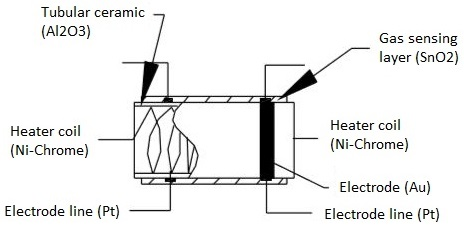
\includegraphics[width=1.0\textwidth]{Sensing-Element-in-Gas-Sensor.jpg}
\end{figure}

Most sensors of the MQ series operate with working voltages that are typically at 5V, and have a lower absorption of 1 watt (5V here means less than 200 milliampere); such an absorption is mainly due to the heating element drawing power. As for some MQ sensors, the heater is powered at 2V: a low and atypical voltage, that we might obtain by using a PWM technique, starting at 5V; in practice we would drive a pulse heater (whose pulse length would be varied), along with a circuit that is based on a PWM modulator. In theory, we should be able to generate 5 V pulses with a 40\% duty-cycle, by means of such a solution.

\begin{figure}
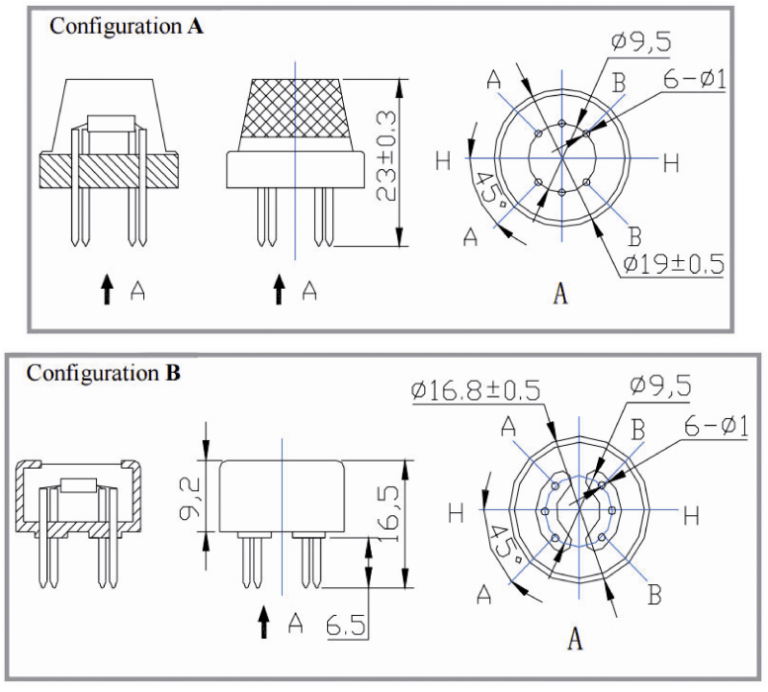
\includegraphics[width=1.0\textwidth]{MQ-X.png}
\end{figure}

The sensors of the MQ series are mainly used in closed environments that anyway should not be particularly cold or warm,\footnote{We should define what hot and cold mean!} given that the heating filament's temperature is kept quite constant by its resistance variation (it grows when the temperature grows, and vice versa) but it is not stabilized nor controlled by any circuit, therefore if the environment is too cold or warm, the obtained measurement would turn out to be altered.

\begin{figure}
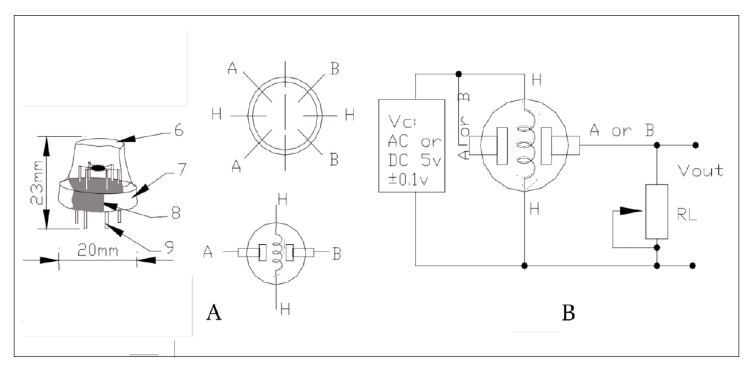
\includegraphics[width=1.0\textwidth]{MQ-X2.png}
\end{figure}

Each sensor of the series reacts to more than one gas, even if usually only one or two gases excite it the most, and supply relevant resistance variations, as it is shown by the sensitivity graphs shown in these pages.


\href{https://playground.arduino.cc/Main/MQGasSensors/#list}{List of sensors and characteristics (Source: playground.arduino)}

\begin{table}
\caption{MQ-X Sensor Parameters }
\begin{tabular}{lp{8cm}cc}\hline
Sensor  & Parameter       & Heater voltage   & Response \\ \hline\hline
MQ-2 & Flammable gases such as LPG and propane & & \\
MQ-3 & Ethanol && \\
MQ-4 & Methane (CH4) and natural gas && \\
MQ-5 & LPG and methane && \\
MQ-6 & LPG and methane && \\
MQ-7 & Carbon monoxide (CO) and Hydrogen (H2) && \\
MQ-8 & Hydrogen (H2) && \\
MQ131 & Ozone & 6 volts & \\
MQ-135 & Gaseous ammonia (NH3), benzene, ethyl alcohol and carbon dioxide (CO2) && \\
MQ136 & Hydrogen Sulphide gas  && \\
MQ137 & Ammonia  && \\
MQ138 & Benzene, Toluene, Alcohol, Propane, Formaldehyde gas, Hydrogen  && \\
MQ214 & Methane, Natural Gas  && \\
MQ216 & Natural gas, Coal Gas  && \\
MQ303A & Alcohol, Ethanol, smoke  && \\
MQ306A & LPG, butane  && \\
MQ307A &  Carbon Monoxide  && \\
MQ309A & Carbon Monoxide, flammable gas  && \\
MG811 (Carbon Dioxide (CO2)) && \\
AQ-104 (air quality) && \\
AQ-2 (Flamable gasses, smoke) && \\
AQ-3 (Alcohol, Benzine) && \\
AQ-7 (Carbon Monoxide) && \\
\hline
\end{tabular}
\end{table}

\subsubsection{Resistance Response}

\begin{equation}
ppm = a\bigg( \frac{R_s}{R_o}\bigg)^b
\end{equation}

\subsubsection{Pin-outs}

These sensors are normally available as modules, these modules consist of the gas sensor and a comparator IC. The pin description of the gas sensor module which we will can use with the Raspberry Pi. The gas sensor module basically consists of 4 terminals

\begin{description}
  \item[Vcc] Power supply
  \item[GND] Power supply
  \item[Digital output] This pin gives an output either in logical high or logical low (0 or 1) that means it displays the presence of any toxic or combustible gases near the sensor. Using this will give an digital output from this pin, by setting a threshold value using the potentiometer. Note: A potentiometer is a three-terminal resistor with a sliding or rotating contact that forms an adjustable voltage divider. If only two terminals are used, one end and the wiper, it acts as a variable resistor or rheostat.
  \item[Analog output] This pin gives an output continuous in voltage which varies based on the concentration of gas that is applied to the gas sensor.
\end{description}


\subsubsection{Coupling to a microcontroller}
Now, let's see how to read the values provided by the sensors, by coupling them to a microcontroller that is supplied with an A/D converter: in order to enable the reading of the sensor's resistance, it is needed to connect a resistor having an opportune value (the higher it is, the wider are the voltage variations, the sensor element's resistance being equal) to the sensor element, in series; after that, let's connect an A pin to the power and a B one to the microcontroller's ADC input, that we will bring to ground by means of a pull-down resistor, as shown in figure With such a connection diagram, that corresponds to the creation of a voltage divider, we obtain – at the resistor's ends – a voltage that is directly proportional to the concentration of gas and aerosol, that depends on the ratio between the sensitive element's resistance and the one of the resistor, and on the basis of the following relationship:

\begin{equation} 
V_u = \frac{Vcc \cdot R}{(R+R_s)}
\end{equation}
 
in which $V_u$ is the voltage at the ends of the load resistor $R$, while $Vcc$ is the sensor's power voltage, and $Rs$ is the electrical resistance of the sensitive element.

\section{Sensor Applications}

\begin{description}

\item[Particulate Matter]

\item[NOx]

\item[O3]

\begin{itemize}
  \item CJMCU-131 Ozone Concentration Sensor High And Low Concentration O3 Air Quality Detection Module
  \item MQ-131
  \item 3SP\_O3\_20 P Ozone Sensor
\end{itemize}

\item[CO]

\item[Pressure, Temperature and Humidity]

\begin{itemize}
  \item BME680 is refered to as a low power gas, pressure, temperature \& humidity sensor, the BME680 is \ldots
  \item DHT11
  \item DHT22
\end{itemize}

The DHT11 and DHT22 sensors can measure humidity as well as temperature. Only one GPIO is used. The difference between the two is mainly the measuring range and accuracy. The white DHT22 can measure all humidity ranges from 0-100\% with an accuracy of 2\%. By comparison, the DHT11 (blue) is only able to measure areas of 20-90\% humidity and above all, the accuracy is significantly worse with 5\%. The light blue DHT11 sensor has a small price advantage (about one buck).

For more information

\begin{itemize}
  \item \href{https://tutorials-raspberrypi.com/raspberry-pi-measure-humidity-temperature-dht11-dht22/}{Raspberry Pi DHT11-DHT22 Tutorial} available on the Raspberry Pi Foundation website.
  \item \href{https://cdn-shop.adafruit.com/product-files/3660/BME680.pdf}{BME680 Data Sheet}
\end{itemize}


\end{description}



\end{document}
